\PassOptionsToPackage{unicode=true}{hyperref} % options for packages loaded elsewhere
\PassOptionsToPackage{hyphens}{url}
%
\documentclass[english,,man,floatsintext]{apa6}
\usepackage{lmodern}
\usepackage{amssymb,amsmath}
\usepackage{ifxetex,ifluatex}
\usepackage{fixltx2e} % provides \textsubscript
\ifnum 0\ifxetex 1\fi\ifluatex 1\fi=0 % if pdftex
  \usepackage[T1]{fontenc}
  \usepackage[utf8]{inputenc}
  \usepackage{textcomp} % provides euro and other symbols
\else % if luatex or xelatex
  \usepackage{unicode-math}
  \defaultfontfeatures{Ligatures=TeX,Scale=MatchLowercase}
\fi
% use upquote if available, for straight quotes in verbatim environments
\IfFileExists{upquote.sty}{\usepackage{upquote}}{}
% use microtype if available
\IfFileExists{microtype.sty}{%
\usepackage[]{microtype}
\UseMicrotypeSet[protrusion]{basicmath} % disable protrusion for tt fonts
}{}
\IfFileExists{parskip.sty}{%
\usepackage{parskip}
}{% else
\setlength{\parindent}{0pt}
\setlength{\parskip}{6pt plus 2pt minus 1pt}
}
\usepackage{hyperref}
\hypersetup{
            pdftitle={Describing vocalizations in young children: A big data approach through citizen science annotations},
            pdfborder={0 0 0},
            breaklinks=true}
\urlstyle{same}  % don't use monospace font for urls
\usepackage{graphicx,grffile}
\makeatletter
\def\maxwidth{\ifdim\Gin@nat@width>\linewidth\linewidth\else\Gin@nat@width\fi}
\def\maxheight{\ifdim\Gin@nat@height>\textheight\textheight\else\Gin@nat@height\fi}
\makeatother
% Scale images if necessary, so that they will not overflow the page
% margins by default, and it is still possible to overwrite the defaults
% using explicit options in \includegraphics[width, height, ...]{}
\setkeys{Gin}{width=\maxwidth,height=\maxheight,keepaspectratio}
\setlength{\emergencystretch}{3em}  % prevent overfull lines
\providecommand{\tightlist}{%
  \setlength{\itemsep}{0pt}\setlength{\parskip}{0pt}}
\setcounter{secnumdepth}{0}

% set default figure placement to htbp
\makeatletter
\def\fps@figure{htbp}
\makeatother

% Manuscript styling
\usepackage{upgreek}
\captionsetup{font=singlespacing,justification=justified}

% Table formatting
\usepackage{longtable}
\usepackage{lscape}
% \usepackage[counterclockwise]{rotating}   % Landscape page setup for large tables
\usepackage{multirow}		% Table styling
\usepackage{tabularx}		% Control Column width
\usepackage[flushleft]{threeparttable}	% Allows for three part tables with a specified notes section
\usepackage{threeparttablex}            % Lets threeparttable work with longtable

% Create new environments so endfloat can handle them
% \newenvironment{ltable}
%   {\begin{landscape}\begin{center}\begin{threeparttable}}
%   {\end{threeparttable}\end{center}\end{landscape}}
\newenvironment{lltable}{\begin{landscape}\begin{center}\begin{ThreePartTable}}{\end{ThreePartTable}\end{center}\end{landscape}}

% Enables adjusting longtable caption width to table width
% Solution found at http://golatex.de/longtable-mit-caption-so-breit-wie-die-tabelle-t15767.html
\makeatletter
\newcommand\LastLTentrywidth{1em}
\newlength\longtablewidth
\setlength{\longtablewidth}{1in}
\newcommand{\getlongtablewidth}{\begingroup \ifcsname LT@\roman{LT@tables}\endcsname \global\longtablewidth=0pt \renewcommand{\LT@entry}[2]{\global\advance\longtablewidth by ##2\relax\gdef\LastLTentrywidth{##2}}\@nameuse{LT@\roman{LT@tables}} \fi \endgroup}

% \setlength{\parindent}{0.5in}
% \setlength{\parskip}{0pt plus 0pt minus 0pt}

% \usepackage{etoolbox}
\makeatletter
\patchcmd{\HyOrg@maketitle}
  {\section{\normalfont\normalsize\abstractname}}
  {\section*{\normalfont\normalsize\abstractname}}
  {}{\typeout{Failed to patch abstract.}}
\makeatother
\shorttitle{Children's vocalizations and citizen science}
\author{Chiara Semenzin\textsuperscript{1}, Lisa Hamrick\textsuperscript{2}, Amanda Seidl\textsuperscript{2}, Bridgette Kelleher\textsuperscript{2}, \& Alejandrina Cristia\textsuperscript{1}}
\affiliation{
\vspace{0.5cm}
\textsuperscript{1} Laboratoire de Sciences Cognitives et de Psycholinguistique, Département d'Etudes cognitives, ENS, EHESS, CNRS, PSL University\\\textsuperscript{2} Purdue University}
\authornote{AC acknowledges Agence Nationale de la Recherche (ANR-17-CE28-0007 LangAge, ANR-16-DATA-0004 ACLEW, ANR-14-CE30-0003 MechELex, ANR-17-EURE-0017); and the J. S. McDonnell Foundation Understanding Human Cognition Scholar Award. LH acknowledges the National Institute of Deafness and Other Communication Disorders (F31DC018219). BK acknowledges the National Institute of Mental Health (K23MH111955) and the Kinley Trust. The funders had no impact on this study.  All authors approved the final manuscript as submitted and agree to be accountable for all aspects of the work and have no conflict of interests to disclose.


Correspondence concerning this article should be addressed to Alejandrina Cristia, 29 rue d'Ulm, 75005, Paris, France. E-mail: alecristia@gmail.com}
\usepackage{lineno}

\linenumbers
\usepackage{csquotes}
\usepackage{setspace}
\AtBeginEnvironment{tabular}{\singlespacing}
\AtBeginEnvironment{lltable}{\singlespacing}
\AtBeginEnvironment{tablenotes}{\singlespacing}
\captionsetup[table]{font={stretch=1.5}}
\captionsetup[figure]{font={stretch=1.5}}
\ifnum 0\ifxetex 1\fi\ifluatex 1\fi=0 % if pdftex
  \usepackage[shorthands=off,main=english]{babel}
\else
  % load polyglossia as late as possible as it *could* call bidi if RTL lang (e.g. Hebrew or Arabic)
  \usepackage{polyglossia}
  \setmainlanguage[]{english}
\fi

\title{Describing vocalizations in young children: A big data approach through citizen science annotations}

\date{}

\abstract{
\textbf{Purpose:} Recording young children's vocalizations through wearables is a promising method. However, accurately and rapidly annotating these files remains challenging. Online crowdsourcing with the collaboration of citizen scientists could be a feasible solution. In this paper, we assess the extent to which citizen scientists' annotations align with those gathered in the lab for recordings collected from young children. \newline

\textbf{Method:} Segments identified by LENA\textsuperscript{TM} as produced by the key child were extracted from one daylong recording for each of 20 participants: 10 low-risk control children and 10 children diagnosed with Angelman syndrome, a neurogenetic syndrome characterized by severe language impairments. Speech samples were annotated by trained annotators in the laboratory as well as by citizen scientists on Zooniverse. All annotators assigned one of five labels to each sample: Canonical, Non-Canonical, Crying, Laughing, and Junk. This allowed the derivation of two child-level vocalization metrics: the Linguistic Proportion, and the Canonical Proportion.
\newline

\textbf{Results:} At the segment level, Zooniverse classifications had moderate precision and recall. More importantly, the Linguistic Proportion and the Canonical Proportion derived from Zooniverse annotations were highly correlated with those derived from laboratory annotations.
\newline

\textbf{Conclusion:} Annotations obtained through a citizen science platform can help us overcome challenges posed by the process of annotating daylong speech recordings. Particularly when used in composites or derived metrics, such annotations can be used to investigate early markers of language delays in non-typically developing children.
}

\begin{document}
\maketitle

TODO

\begin{itemize}
\tightlist
\item
  create OSF for this paper specifically
\item
  references!
\item
  merge noncan/can for LENA\textsuperscript{TM} in Table 1
\item
  appropriately merge col names in tab 1
\item
  add 2 explo analyses that are still missing
\item
  Redo pipeline so that it's transparent \& integrated
\end{itemize}

Language production at 3 years of age is the best predictor of later academic and economic achievement (Law et al., 2003). Early language delays can adversely affect children's literacy, behavior, social interaction, and scholastic achievement extending well into adulthood, with early interventions being a better societal investment than later ones (Heckman, 2006). Advancements in the field of wearable technologies, such as LENA\textsuperscript{TM} recorders, have opened new avenues to both early detection of speech pathologies and research in language development more generally. Wearable recorders allow data collection to happen in the child's natural environment, and at a large scale, which may be particularly helpful for children whose speech is not easily elicited. Although such long-form recordings are increasingly common REF, challenges remain with respect to how these data are handled, annotated, and analyzed. The present work reports on the validity of labels and child-level descriptors of children's vocalizations gathered from citizen scientists, in a comparison to expert lab annotators. In the rest of the Introduction, we first briefly summarize two metrics that can be used to describe individual children's vocalizations in the context of long-form recordings. We then introduce crowdsourcing in general, and crowdsourcing by citizen scientists in particular, as a potential avenue for more rapidly deriving these key metrics from vocalization recordings.

\hypertarget{describing-childrens-vocalizations-in-long-form-recordings}{%
\subsubsection{Describing children's vocalizations in long-form recordings}\label{describing-childrens-vocalizations-in-long-form-recordings}}

A large body of research has investigated both fine-grained and coarse descriptions of children's vocalizations as a function of age and diagnosis, and it is beyond the scope of this paper to provide a full summary of this work. We instead focus on two descriptors -- Linguistic Proportion and Canonical Proportion -- that are particularly amenable to the kind of big data approaches long-form recordings require.

To understand why these two descriptors are relevant, it is worthwhile to first consider how the way in which vocal development has been studied in the past may not easily translate to long-form recordings. As mentioned earlier, long-form recordings have several advantages, including capturing the child's vocal patterns in their natural environment and being able to accumulate a great amount of data easily, which is particularly useful for diagnoses and pathologies characterized by low levels of vocal production. However, this also means that there is a great amount of data, and that the audio quality is compromised, as children go about their day transitioning from small to large rooms, with fewer or more people around them, thus providing analysts with an unstable and challenging long audio. In fact, human annotation of such audio is estimated to take about 30 times the audio length, with these estimates being greater the more precise one wants or needs to be (Seidl et al., 2019). It is for this reason that most users of long-form recordings have turned to automatized software for at least a first-pass analysis.

The most commonly used software was created by the LENA\textsuperscript{TM} Foundation, and it returns a diarization of the audio signal split into key talkers, including the child wearing the device, as well as a split of these audio attributed to the child into three categories: crying, other fixed and vegetative signals, and speech vocalizations. These subcategories have not been widely validated (Cristia et al., 2020). To provide an idea of their accuracy, we classified the same segments that are used in the present study using LENA\textsuperscript{TM}'s subtypes\footnote{If a child segment contained speech, then it counted towards canonical/non-canonical; else, if it contained crying it counted towards crying; else, if it contained some fixed signals it counted towards laughing; a small proportion were left that did not have any of the three and were considered as \enquote{junk} or not categorized.} to compared these against the laboratory annotations used in the present study. Table 1 shows that LENA\textsuperscript{TM} has a good recall for speech-like vocalizations and crying but not laughing. Moreover, LENA\textsuperscript{TM} lacks an important distinction between more and less advanced vocalizations.

\begin{table}

\caption{\label{tab:tab-LENA-challenge}Comparison of recall percentages obtained with the baseline algorithm created by the ComParE team, in the context of the ComParE 2019 BabySounds subchallenge (Schuller et al., 2019), LENATM labels (note LENATM does not distinguish between Canonical and Non-canonical), and those obtained in this study through Zooniverse annotations. Label frequency indicates the prevalence of the relevant label (Crying, Laughing, etc.) in each dataset (the same Lab dataset was used for both LENATM and Zooniverse). UAR stands for unweighted average recall, WAR for weighted average recall (which takes into account label frequency).}
\centering
\begin{tabular}[t]{l|l|l|l|l|l}
\hline
 & Recall &  &  & Label & Frequency\\
\hline
 & C2019B & LENA & Zoon. & C2019B & Lab\\
\hline
Crying & 70.6 & 78.0 & 49.0 & 669 & 581\\
\hline
Laughing & 41.5 & 12.0 & 56.0 & 149 & 137\\
\hline
Non-can. & 24.1 & 73.0 & 77.0 & 4485 & 5512\\
\hline
Canonical & 66.4 &  & 59.0 & 1426 & 1715\\
\hline
Junk & 67.3 & 1.0 & 44.0 & 4575 & 2169\\
\hline
UAR & 54.0 & 41.0 & 57.0 &  & \\
\hline
WAR & 49.9 & 57.0 & 65.0 &  & \\
\hline
\end{tabular}
\end{table}

Other automatized algorithms have been developed in recent years, saliently ones attempting to classify child vocalizations into crying, laughing, canonical, and non-canonical (Schuller et al., 2019). The split of speech vocalizations into canonical and non-canonical, and the overt inclusion of laughing, allow a somewhat finer-grained picture of children's vocal activity. An advantage of these algorithms is that there exists a challenge where performance has been benchmarked, so unlike LENA\textsuperscript{TM}'s algorithms, we know which algorithms perform better than others. The ComParE 2019 BabySounds sub-challenge established a state-of-the-art baseline with a test-set unweighted average recall of around 55\% (see Table 1). The team who won the challenge improved this by about 2\%, primarily through gains in the laughing class obtained by adding training data (REF). Given that the laughing class is very rare, improvements in this class do not mean that performance as a whole, when all classes are considered, changes very much.

One possibility that has only recently begun to be explored is the use of derived metrics. So instead of evaluating algorithms and other annotation procedures on their accuracy at individual labels, one can derive a metric that more closely relates to vocalization development.

For example, most work using LENA\textsuperscript{TM} software reports on children's vocalization counts. Although this has been sometimes criticized as being more about quantity than quality REF, this is a promising metric because it shows correlations with age (which is a proxy of development), and it can be extracted quite accurately with LENA\textsuperscript{TM} REF. Additionally, the child vocalization count metric has been found to be concurrently and predictively correlated with an effect size r \textasciitilde{} .3 with standardized language scores in a meta-analysis REF. Thus despite representing a composite of skills, vocalization count may provide a useful estimate of vocalization development.

Here, we focus on two alternative composite metrics. An additional metric that can be derived once children's vocalizations are split into crying, laughing, canonical, and non-canonical is the Linguistic Proportion: the proportion of vocalizations that are linguistic (canonical and non-canonical) out of all vocalizations. To our knowledge, this metric has not been extensively explored previously, but it is likely that this proportion increases with age REF.

Yet another metric that could be extracted to estimate relative linguistic complexity is the Canonical Proportion: the proportion of vocalizations that are canonical out of all linguistic (canonical and non-canonical) vocalizations. One recent study has established that the Canonical Proportion extracted from daylong recordings is significantly correlated with age in a multicultural and multilingual sample REF. Importantly, this association was established in a sample of children going up to 3 years of age, and thus well beyond the babbling period, and into first words and word combinations.

There is a wider research base documenting the potential importance of the Canonical Proportion, and related metrics, although this work focuses on babbling and thus typically on infants under one year of age. A critical milestone involves the increasingly common production of Canonical Syllables, consonant-vowel (CV) or vowel-consonant (VC) sequences that resemble those found in adult speech (Oller et al., 1998). Given its adult-like CV or VC structure, canonical babble is considered to be a starting point on the path to recognizable speech. Canonical syllables show a higher complexity given the smooth articulatory transition between a consonant and a vowel (or vice versa), when compared to more primitive sounds such as squeals, or isolated vowels. Some work suggests that Canonical Proportions above .15 are expected by about 10 months of age in typical development (Oller et al., 1999). In addition, delayed onset of canonical babbling has been documented in a wide variety of disorders and delays (Belardi et al., 2017; Fasolo et al., 2008; Lang et al., 2019; Patten et al., 2014; Stoel-Gammon, 2016).

In sum, there is a growing literature attempting to use data from daylong recordings to describe young children's vocalizations, but there are two outstanding challenges. The first pertains to how the data are analyzed, with human annotation being costly. The second relates to how to extract useful descriptors, both in terms of individual vocalizations and at the child level.

\hypertarget{crowdsourcing-a-potential-solution-for-annotation}{%
\subsubsection{Crowdsourcing: A potential solution for annotation}\label{crowdsourcing-a-potential-solution-for-annotation}}

Crowdsourcing refers to the process whereby a task is solved by a crowd, rather than an individual. A number of fields, particularly in the data-driven sciences, have already engaged in the collection of data (including annotations) through crowdsourcing, thanks to its low cost and ecological value (Crump, McDonnell, \& Gureckis, 2013; Sescleifer, Francoisse, \& Lin, 2018; Sprouse, 2011). For example, a systematic review on crowd-sourced ratings of speech (Sescleifer et al., 2018) found that \enquote{lay ratings are highly concordant with expert opinion, validating crowdsourcing as a reliable methodology}; across studies, crowdsourced and expert listener classifications yielded a mean correlation coefficient of .81. On the other hand, the systematic review returned only 8 studies (of which only four were published in peer-reviewed journals), suggesting that there is considerable need for further research on this topic.

Mechanical Turk (MTurk) MTurk is an online labor market created by Amazon to assist \enquote{requesters}'\enquote{" in hiring and paying \enquote{workers} for the completion of computerized tasks. Although it is a leading crowdsourcing service, and some evidence suggests MTurkers} annotations can be quite reliable (Berinsky et al., 2012), some question marks are raised as some \enquote{workers'} turn out to be bots, or poorly motivated (and potentially exploited).

A promising crowd-sourcing alternative has arisen in recent years: citizen science, a research technique that engages the public in the collection of scientific information (ref). As citizen scientists do not receive compensation, this alternative to platforms such as MTurk can overcome the limitations posed by potential exploitation of workforce and/or the use of bots. Volunteers are entirely motivated by the desire to contribute to research advancements as well as the pleasure they derive from the task itself.

One of the most successful platforms hosting citizen science projects is Zooniverse (zooniverse.org). The website hosts a multitude of interdisciplinary projects that have allowed the public to take part in cutting-edge scientific research, from marine biology to papyrology. Zooniverse has proven extremely useful in those fields where the complexity of the data collected is too high to be automatically interpreted using computer algorithms (ref) At the same time, the tasks that human volunteers are asked to complete are sufficiently simple that citizens can carry them out without a background in science or any extensive training (ref).

Citizen science may be particularly helpful when analyzing infants' data from wearables, which remain challenging to annotate as mentioned above. There is one previous study that attempted this approach. Cychosz et al. (2019) drew child vocalization data from a diverse set of corpora centered on children learning one of four languages: English, Tseltal, Tsimane', and Yélî. For the English and Tsimane' corpora, vocalizations were automatically identified using LENA\textsuperscript{TM}, whereas the other two were extracted through manual segmentation. Vocalizations were split into maximally 500-ms long clips, and presented to annotators through the citizen science iHearUPlay platform, with the aim that each clip received 3 classifications into crying, laughing, canonical, non-canonical, or \enquote{junk} (with the latter tag used for clips that did not contain clear child voice). They then derived an implementation of the Canonical Proportion, as the proportion of clips receiving a majority judgment of canonical out of the clips receiving a majority judgement of canonical or non-canonical. They found that this canonical ratio increased with infant age in an analysis collapsing across corpora, which provides a first proof of principle that citizen scientists' annotations could be an appropriate solution to the problem of annotating child vocalizations from wearables. The authors also studied how their canonical ratio related to age within each corpus that had a sufficient number of children varying in age. They found that in one English corpus bearing on very young infants, the proportion of clips assigned to the \enquote{junk} category was very high. Additionally, they found that the correlation between canonical ratio and age was much weaker in two corpora where vocalizations were segmented with LENA\textsuperscript{TM} than through manual segmentation. In sum, these analyses within corpora reveal that data may not be uniformly useful, with potential variation across corpora, children, and methods.

\hypertarget{the-present-work}{%
\subsubsection{The present work}\label{the-present-work}}

Our work seeks to broaden the already promising results that have emerged from previous work summarized above. We hope that this methodology will open the road to larger scale analyses of children's vocalizations as captured by wearables. In addition, we went beyond Cychosz et al. (2019)\enquote{s study in two important ways. First, we relied on the largest and best established citizen science platform: Zooniverse hosts more than 1.6 million users from diverse walks of life, and it offers a completely automatized API system to more easily scale tasks in a transparent and cumulative science fashion. In contrast, the authors of that paper told us that, in order to complete their data annotation, they recruited the help of students in their classes and labs, and sometimes the researchers themselves took on a considerable annotation load. This means that the process draws on expert resources, whose time is expensive. Moreover, the people these researchers recruit tend to be more accustomed to child vocalization data, which may improve their annotation performance, and thus provide an overestimate of the quality of the annotations that can be realistically done within a truly citizen science framework. Those authors also had to rely on manual extraction of the resulting data from the iHearUplay team, which added to the administrative load. Second, a core goal of the present work was to determine how citizen scientists} annotations fare compared to the current gold standard, laboratory annotations. Cychosz et al. (2019) did not have a gold standard for their data.

Thus, the present study aimed to contribute a key piece of evidence missing in this discussion: To what extent do laboratory and citizen science annotations agree when describing young children's vocalizations? We examined the extent to which such classifications agree, by quantifying the correspondence across these two modes of annotations at the level of individual clips (vocalizations), and at the level of individual children. It was important for generalizability purposes to examine data from children with variable biological, mental age, and vocal maturity levels. We therefore included children in a wide age range, with some of the children being diagnosed with Angelman Syndrome, as well as low-risk controls.

At the segment level, we checked the extent to which laboratory annotations made by experts agreed with judgments made by citizen scientists. We used confusion matrices to describe annotation convergence and divergence patterns, and overall accuracy, kappa, and Gwet's AC1 coefficient as statistical descriptors. Given previous results from machine learning classifiers REF, we expected agreement to be moderate at this level, with potentially more erratic results for categories that are rarer.

When considering correspondence at the level of individual children, we derived two metrics: the Linguistic Proportion (canonical+non-canonical)/(all vocalizations); and the Canonical Proportion (canonical)/(all linguistic vocalizations). Previous work suggests that children with Angelman Syndrome show decreases in Canonical Proportion with age, whereas in typically-developing infants, conversely, the canonical ratio was expected to increase with age (Hamrick, Seidl, \& Kelleher, n.d.). Although we could not rely on previous work to make predictions regarding the Linguistic Proportion, we reasoned that we should observe an increase in the Linguistic Proportion for both populations.

More specific to our research aims, we checked the degree to which laboratory and citizen science annotations converged at the child level by using correlations across the two. We additionally explored under what conditions Zooniverse judgments are more closely aligned with laboratory judgments using linear mixed models.

\hypertarget{methods}{%
\subsection{Methods}\label{methods}}

All analyses and key data are available for reproduction on OSF (\url{https://osf.io/57yha/}). Computer code used to collect the Zooniverse judgments is available from GitHub (Semenzin, 2020).

\hypertarget{participants}{%
\subsubsection{Participants}\label{participants}}

The full data set includes data from 20 children: 10 English-speaking children (6 males, 4 females; age range 11-53 months, mean=41.5 months) diagnosed with Angelman syndrome (AS) and 10 low-risk control (LRC) children (6 males, 4 females; age range 4-18 months, mean=11.7 months). As children diagnosed with Angelman syndrome typically have severe cognitive and language delays and most do not produce more than 1-2 words consistently, we compare their linguistic production data against that of younger children with theoretically similar language profiles.

\hypertarget{equipment-and-data-collection-procedure}{%
\subsubsection{Equipment and data collection procedure}\label{equipment-and-data-collection-procedure}}

Recordings were obtained with the Language ENvironment Analysis (LENA\textsuperscript{TM}) Digital Language Processor, LENA\textsuperscript{TM} is a lightweight recorder (\textless{} 60 g, 5.5 cm x 8.5 cm x 1.5 cm) designed to be worn inside a breast-pocket of purpose-made clothing. In our data, every child contributed at least one daylong recording, with one child contributing two recordings (duration 11.58-16.00 hours, mean 15.05 hours).

\hypertarget{data-preprocessing-lenatm}{%
\subsubsection{\texorpdfstring{Data preprocessing (LENA\textsuperscript{TM})}{Data preprocessing (LENATM)}}\label{data-preprocessing-lenatm}}

The first step we took before beginning the annotation process was the identification of children's vocalizations within day-long recordings. We did this automatically, using the LENA\textsuperscript{TM} proprietary software. Specifically, the LENA\textsuperscript{TM} software attempts to assign segments of speech either to the key child (the one wearing the recorder), or to one of 15 other categories in the child's environment (e.g., Female-Adult, TV). Key child labels have a precision of about XX\% and a recall of about XX\% (ref). These stretches of audio assigned to the key child can contain cries, vegetative sounds, and linguistic vocalizations, as well as interstitial pauses. We will refer to them as segments, to highlight the fact that they are stretches of audio segmented out as belonging to the key child, but they may not be individual vocalizations.

\hypertarget{annotation-by-lab-experts}{%
\subsubsection{Annotation by lab experts}\label{annotation-by-lab-experts}}

Annotation was carried out at the segment level during lab coding. A subset of segments LENA\textsuperscript{TM} identified as the key child were selected for human annotation. Segments were selected from 30 five-minute sections of the child's recording: 10 sections during which the child was vocalizing at their highest rate, and 20 sections drawn randomly from the remainder of the recording. To ensure generalizability of our data, we included in this subset a number of segments of audio coming from both periods of high child volubility, as well as randomly selected periods of the day.

Annotations were carried out by 20 undergraduate students working in either Speech, Language, and Hearing Sciences or clinical psychology laboratories. Before annotation, coders completed an ethical conduct of research course and received HIPAA compliance training. After this, they complete a brief training on vocal maturity that involves 1) reading relevant literature, 2) reviewing examples of various annotation categories and 3) completing a brief quiz to test their annotation accuracy. Coders then proceed to the classification, where they make decisions on whether a segment is a cry, laugh, non-canonical syllable(s), canonical syllable(s), or a word. Coders are instructed to classify each segment based on the highest level of vocal maturity it contains (e.g., a segment with both canonical and non-canonical syllables would be classified as canonical; a segment with both laughing and non-canonical syllables would be classified as non-canonical). For canonical, non-canonical, and word segments, coders indicated how many syllables of each type of vocal maturity they hear (e.g., \enquote{ah ma ba} would be 1 non-canonical and 2 canonical syllables). Coders are also given a \enquote{Don't Mark} option, which they are instructed to use if the segment does not sound like a segment made by the target child, or if there is any overlapping speech or other noise in the background which could affect acoustic analyses. For the purposes of the present study, we considered a \enquote{word} judgment to be equivalent to a \enquote{canonical} judgment. This may be false sometimes (e.g., \enquote{oh} may be coded as a real word by laboratory experts, although it is a non-canonical syllable), but we could not have a \enquote{word} judgment in our Zooniverse annotations because that requires context (which compromises privacy -- see next section). This process resulted in high levels of agreement: 97.22\% of the lab-annotated segments had either 2 or 3 coders agree.

\hypertarget{annotation-on-zooniverse}{%
\subsubsection{Annotation on Zooniverse}\label{annotation-on-zooniverse}}

A substantial concern that emerges when considering citizen science annotation for spontaneous speech data is the risk of a privacy breach: even short clips can contain personal information that can expose the identity of the speaker, such as addresses or names, or contain sensitive and private information. Fortunately, a study by Seidl et al. (2019) determined that when segments are divided into shorter chunks (400-600ms), human annotators can code our categories of interest (canonical, laughing, crying, etc.) with a classification quality comparable to the one carried out on full segments. We therefore used very short chunks (500ms) as these are unlikely to contain more than two syllables, and thus prevent the identification of any personal information.

Specifically, the segments extracted were automatically cut into clips of exactly 500ms, extracting neighboring silence when necessary, before being uploaded on the Zooniverse platform. To allow the recovery of the original segments at later stages of the analysis, the scripts created a metadata file with the mapping between 500ms clips and their corresponding segment. Clips were then uploaded on Zooniverse using Panoptes, their open-source, command-line based API for data handling (\url{https://github.com/zooniverse/panoptes-cli}).

Citizen scientists could access the project by logging in, or as anonymous participants. Before starting the annotation, participants were given a quick tutorial which walked them through the steps of the annotation workflow (i.e., how to play a sound, how to make a selection; see Figure 1). In this tutorial, we included one audio example for each category in order to make the classification task as smooth as possible. Further clarifications on what constitutes Canonical and Non-canonical utterances, as well as five audio examples for each of the categories, were available through the Field Guide, which users could access by clicking on the right side of the screen. The Field Guide could be consulted at any point of the classification without interrupting the task.

Users were asked to assign each 500ms clip to one out of five possible categories: (1) canonical, (2) non-canonical, (3) crying, (4) laughing, and (5) junk (overlapping speech, non-infant speech, silence, external sounds). Notice that the latter is narrower than the \enquote{Don't mark} category of the lab annotation routine, which was used any time there was noise or overlap that could affect acoustic analyses.

Following recommendations from the Zooniverse board, we collected 5 judgments per clip, rather than 3 as used in the laboratory. Majority agreement is thus achieved when 3 out of 5 judgements agree (rather than 2 out of 3). In exploratory analyses, we assess the impact of collecting a smaller number of judgments per clip.

\begin{figure}
\centering
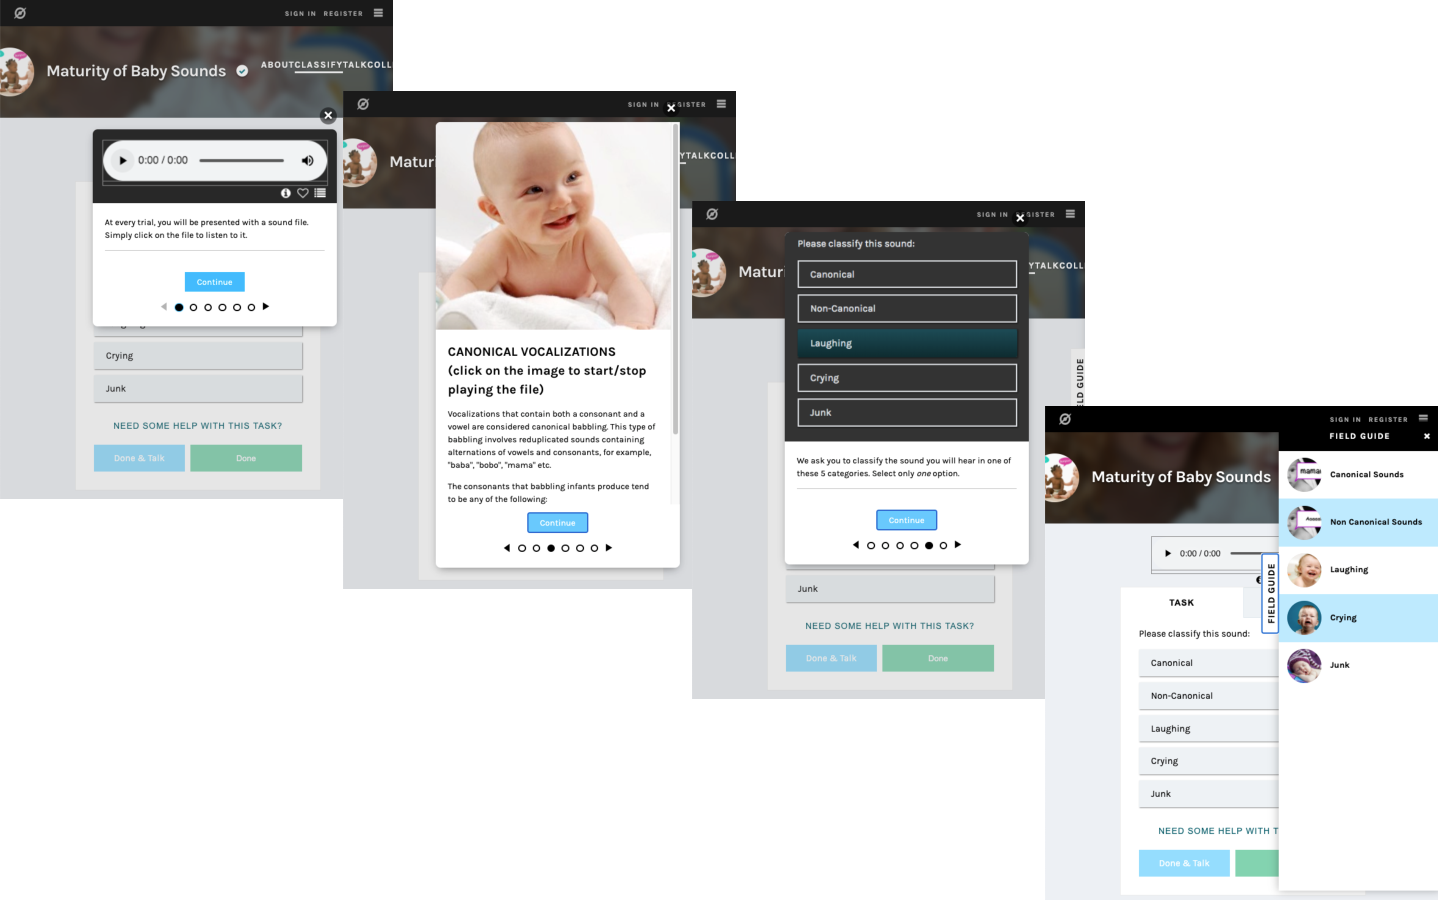
\includegraphics{zooniverse-pufig.pdf}
\caption{\label{fig:fig-zoo}Screen captures of the 6 stages of the tutorial, three of which are shown here: The initial explanation of the trial, examples of canonical vocalizations, and the classification choice the user needs to make; as well as the field guide, which remains accessible on the right of the screen throughout the session, and which allows users to revise examples of the different categories.}
\end{figure}

\hypertarget{data-post-processing}{%
\subsubsection{Data post-processing}\label{data-post-processing}}

An impressive total of 4,825 individual Zooniverse users provided labels for the Maturity of Baby Sounds project, of which the present data set is one part. For this project, we collected a total of 169,767 judgments provided for 33,731 500-ms chunks, corresponding to 11,980 LENA\textsuperscript{TM} segments. Nearly a fifth of chunks did not have at least 3 labels in agreement out of the 5 Zooniverse labels (N = 6,585, 19\% of all chunks). Of the chunks without a majority agreement, 4341 (66\%) contained one or two Junk judgements (out of 5), 6523 (99,9\%) had at least two matching judgements (the threshold used for lab-annotated segments), and only 61 (0,01\%) had 5 different judgements. Future work may explore different ways of setting the minimal requirement for convergence, but for further analyses here, we focused on the 81\% of chunks that did have at least 3 labels in agreement; this represented 135,725 labels for 27,145 chunks, corresponding to 11,593 LENA\textsuperscript{TM} segments. As the segments average 1.12 seconds in length, this means about 3.8 hours of audio data were annotated by 8 different annotators (3 in the laboratory, 5 on Zooniverse).

Lab annotators provided judgments at the level of LENA\textsuperscript{TM} segments, whereas Zooniverse annotators provided judgments on 500 ms chunks, which are typically smaller than the segments. Therefore, we needed to combine chunk-level judgments to reconstruct segment-level judgments.

We did this by considering the majority label extracted from Zooniverse judgements for all chunks associated with each segment, and then following these rules: If the majority label for all chunks associated with a given segment were junk, then the segment was labelled as junk; then, following a hierarchy (Canonical\textgreater{}Non-canonical\textgreater{}Laughing\textgreater{}Crying), segments with at least one instance of each judgement were labelled as such: e.g.~if one canonical judgement was present, then the segment was labelled as canonical, otherwise if a non-canonical judgement was present, the segment was labelled as non-canonical, and so on. This is essentially the same thought process expert annotators followed when labeling segment-level audio, as each segment can represent multiple classification subtypes). LENA\textsuperscript{TM} segments are not equivalent to child vocalizations: A segment may contain 1 or more vocalizations, which may be of the same type or not.

\hypertarget{results}{%
\subsection{Results}\label{results}}

\hypertarget{descriptive-analyses}{%
\subsubsection{Descriptive analyses}\label{descriptive-analyses}}

In this section, we provide descriptive analyses of our dataset. According to lab annotators, 15\% of segments were canonical, 56\% non-canonical, 2\% laughing, and 5\% crying, with the remaining 22\% being categorized as \enquote{Don't mark}. Zooniverse data revealed a similar distribution: 15\% canonical, 60\% non-canonical, 4\% laughing, 9\% crying, 13\% junk.
Next, we inspected the relationship between age and child-level derived metrics, of which we had two: i) Linguistic Proportion = (\enquote{Canonical}+\enquote{Non-Canonical})/\enquote{All vocalizations} (i.e., we remove, junk), and ii) Canonical Proportion = \enquote{Canonical}/(\enquote{Canonical}+\enquote{Non-Canonical}) (i.e., we remove junk + non-linguistic). See Figure 2 for results.

\begin{figure}
\centering
\includegraphics{paper_files/figure-latex/fig-corage-1.pdf}
\caption{\label{fig:fig-corage}Correlations between child-level descriptors and age as a function of metric (linguistic ratio in the top row, canonical ratio in the bottom row), annotation method, and child group (red=low-risk, and black Angelman Syndrome)}
\end{figure}

Descriptive analyses on the laboratory annotations showed that correlations between the Linguistic Proportion and age differed across the groups. There was a near-zero relationship among the older children diagnosed with Angelman Syndrome r(8) = 0.02, CI {[}-0.62,0.64{]}, p=0.97{]}; and a significant association among younger low-risk control children r(8) = 0.74, CI {[}0.21,0.94{]}, p=0.01{]}. The Canonical Proportion exhibited non-significant developmental decreases among older children diagnosed with Angelman Syndrome r(8) = -0.56, CI {[}-0.88,0.11{]}, p=0.09{]}; and marginal developmental increases among low-risk control r(8) = 0.61, CI {[}-0.04,0.90{]}, p=0.06{]}.

Using the Zooniverse annotations, we found that the association with age was very weak for children diagnosed with Angelman Syndrome r(8) = -0.10, CI {[}-0.68,0.57{]}, p=0.79{]}; whereas younger low-risk control children showed a significant increase with age r(8) = 0.68, CI {[}0.08,0.92{]}, p=0.03{]}. Similarly, there were non-significant developmental decreases in the Canonical among children with Angelman Syndrome r(8) = -0.42, CI {[}-0.83,0.29{]}, p=0.23{]}; and marginal developmental increases among low-risk control children, r(8) = 0.60, CI {[}-0.04,0.89{]}, p=0.06{]}.

\hypertarget{main-analyses}{%
\subsection{Main analyses}\label{main-analyses}}

Next, we discuss the correspondence between citizen science classifications and the laboratory gold standard, at the level of individual clips. Results were visualized with a confusion matrix showing precision and recall (Figure 3): the diagonal elements show the number of correct segment-level classifications for each class while the off-diagonal elements show non-matching classifications.

\includegraphics{paper_files/figure-latex/fig-prec-rec-1.pdf}

These visualizations suggest that performance is moderate to good, which was confirmed via statistical analyses. The overall (weighted) accuracy is 65\%, CI = {[}64,66{]}, kappa is 0.43, and the Gwet's AC1 coefficient is 0.59, CI = {[}0.58,0.60{]}.

\hypertarget{child-level-descriptors}{%
\subsubsection{Child level descriptors}\label{child-level-descriptors}}

\includegraphics{paper_files/figure-latex/corlab-zoo-1.pdf}

Although the classification at the clip level is only moderately accurate, what we are ultimately interested in is whether citizen scientists' classifications are able to provide a reliable snapshot of childrens' individual development. Looking at all 20 children together, we found a strong positive correlation r(18) = 0.81, CI {[}0.57,0.92{]}, p=0{]} between Linguistic Proportion by child from the Zooniverse and the lab annotators' data. When we split by participant group, correlations remain high: for Angelman Syndrome r(8) = 0.88, CI {[}0.55,0.97{]}, p=0.00{]}; low-risk control r(8) = 0.82, CI {[}0.40,0.96{]}, p=0.00{]}.

Similarly, a strong positive correlation is found in the Canonical Proportion r(18) = 0.94, CI {[}0.84,0.98{]}, p=0{]}. When we split by participant group, correlations remain high although we do note they are somewhat smaller for the older children with Angelman Syndrome: r(8) = 0.86, CI {[}0.50,0.97{]}, p=0.00{]}; than the low-risk control children r(8) = 0.96, CI {[}0.83,0.99{]}, p=0.

\hypertarget{additional-analyses}{%
\subsection{Additional analyses}\label{additional-analyses}}

We additionally explored under what conditions Zooniverse judgments more closely aligned with laboratory judgments. In previous work using a similar method, for instance, data from all three children from one dataset were often labeled as \enquote{Junk} (i.e., not a child's vocalization), and the data points from this corpus stood out when the authors attempted to integrate results with other corpora (Cychosz et al., 2019). A high proportion of \enquote{Junk} may indicate that automated segmentation was errorful for those children, and may be a sign that the rest of the data could be compromised as well.

\includegraphics{paper_files/figure-latex/cor-junk-1.pdf}

We investigated this hypothesis by calculating the proportion of their data labeled as \enquote{Junk} for each individual child. There was no significant difference in the proportions of their data labeled as \enquote{Junk} for older children with Angelman Syndrome (M = 0.13) compared to the younger low risk children (M = 0.14): Welch's t(13.37) = -0.52, p = 0.61. We therefore collapsed across groups for this exploratory analysis, and split the 20 children using a median split on the proportion of their data labeled as \enquote{Junk}. Results were similar across these two post-hoc subgroups. For Linguistic Proportion, the correlation across lab and Zooniverse data for the lower junk group was r(8) = 0.87, CI {[}0.53,0.97{]}, p=0.00{]}; and for the higher junk group it was r(8) = 0.87, CI {[}0.54,0.97{]}, p=0.00. For Canonical Proportion, the correlation across lab and Zooniverse data for the lower junk group was r(8) = 0.96, CI {[}0.82,0.99{]}, p=0{]}; and for the higher junk group it was r(8) = 0.93, CI {[}0.73,0.98{]}, p=0. Thus, it does not seem that a higher proportion of \enquote{Junk} judgments is an index of low quality data.

Above, we concluded that derived metrics seem more promising than segment-level data. Notice that derived metrics do not require matching of clips (500 ms presented to Zooniverse participants) to segments (the original LENA\textsuperscript{TM} segments presented to laboratory participants). As a result, there was one stage in our pre-processing that may not have been necessary, whereby we collapsed judgments across chunks associated to the same segment. We therefore repeated our analyses but deriving our proportions for the Zooniverse data not from the segment-level composite, but rather the individual chunk-level annotations.

Regarding correlations with age, we found that the Linguistic Proportion was not strongly associated with age in the Angelman Syndrome group: r(8) = -0.04, CI {[}-0.65,0.61{]}, p=0.92{]}, but increased with age in the low-risk control group: r(8) = 0.72, CI {[}0.16,0.93{]}, p=0.02. Similarly, the Canonical Proportion did not exhibit the same pattern across the groups, with developmental decreases found among children with Angelman Syndrome r(8) = -0.38, CI {[}-0.81,0.33{]}, p=0.28{]}; and developmental increases among low-risk control r(8) = 0.57, CI {[}-0.09,0.88{]}, p=0.08.

As for correlations between Zooniverse and laboratory-derived metrics, we observe very similar levels of correlation: Linguistic Proportion overall r(18) = 0.84, CI {[}0.64,0.94{]}, p=0{]} between Linguistic Proportion by child from the Zooniverse and the lab annotators' data. When we split by participant group, correlations remain high: for Angelman Syndrome r(8) = 0.84, CI {[}0.46,0.96{]}, p=0.00{]}; low-risk control r(8) = 0.84, CI {[}0.45,0.96{]}, p=0.00{]}. As for Canonical Proportion overall r(18) = 0.96, CI {[}0.91,0.98{]}, p=0; Angelman Syndrome: r(8) = 0.87, CI {[}0.52,0.97{]}, p=0.00{]}; low-risk control infants r(8) = 0.98, CI {[}0.89,0.99{]}, p=0.

Since all of these results are very similar to those obtained when first matching clips to segments, we conclude that in the future this step may not be necessary. Instead, researchers can derive linguistic and Canonical Proportions directly from citizen scientists' clip level judgements (which was in fact what Cychosz et al., 2019 did).

Next, we looked at whether having more segments from each child may lead to more reliable metrics. We observed a non-significant trend {[}t(17.92)=527.40 and 631.90{]} for lower number of segments in the Angelman Syndrome group (mean 527.40, range 326-924) than among low-risk control infants (mean 631.90, range 351-1074), likely because of the lower volubility of the former children. Moreover, these numbers of segments are much larger than those used in previous work relying on citizen science classifications {[}CITE MEG{]}. We therefore asked whether the correlations between laboratory and Zooniverse child-level estimates are affected by how much data is extracted from each child by sampling 100 segments from all children {[}following CITE MEG{]}. We randomly sampled 100 segments from each child's data, and recalculated the linguistic and Canonical Proportions based only on these associated judgments. We repeated this process 50 times, to assess the extent to which the association between laboratory- and Zooniverse-derived metrics varied in each random sample. The mean correlations across 50 runs were lower than those recovered using all segments from each child (see Table XX), particularly for the low-risk younger infants, and for Linguistic Proportion. This may indicate that, particularly in some groups of infants, 100 segments may not be sufficient to capture the child's linguistic and Canonical Proportions. We also observed quite a bit of variance across the 50 runs. For Linguistic Proportion, the range of correlations found for all infants was {[}0.64,0.88{]}; for the Angelman Syndrome group {[}0.76,0.94{]}; for the low-risk group {[}0.45,0.95{]}. For Canonical Proportion, the range of correlations found for all infants was {[}0.82,0.96{]}; for the Angelman Syndrome group {[}0.40,0.97{]}; for the low-risk group {[}0.75,0.97{]}.

\begin{table}

\caption{\label{tab:tab-cors}Pearson correlation coefficients across metrics derived from laboratory and Zooniverse annotations in the Angelman Syndrome (AS) group data, low-risk (LR) group data, or for all children together (all) in three ways: All seg indicates that Zooniverse annotations at the clip level were first combined at the segment level; Chunks that they were analyzed directly at the clip level. Both of these are based on all the data. In contrast, rows labeled 100 seg indicate that laboratory- and Zooniverse-derived metrics were based on only 100 segments (median over 50 runs in which 100 segments were randomly selected from each child).}
\centering
\begin{tabular}[t]{l|r|r}
\hline
  & Linguistic Proportion & Canonical Proportion\\
\hline
All seg AS & 0.877 & 0.858\\
\hline
All seg LR & 0.823 & 0.960\\
\hline
All seg all & 0.811 & 0.937\\
\hline
Chunks AS & 0.845 & 0.866\\
\hline
Chunks LR & 0.841 & 0.975\\
\hline
Chunks all & 0.845 & 0.963\\
\hline
100 seg AS & 0.857 & 0.807\\
\hline
100 seg LR & 0.806 & 0.892\\
\hline
100 seg all & 0.783 & 0.903\\
\hline
\end{tabular}
\end{table}

\hypertarget{discussion}{%
\subsection{Discussion}\label{discussion}}

In the present study we assessed the extent to which child vocalizations from LENA\textsuperscript{TM} daylong recordings can be accurately described based on classifications collected using the citizen science platform Zooniverse. Our recordings came from children diagnosed with a language disorder, as well as low-risk controls, and included a range of different ages. Excerpts of these recordings had previously been annotated by trained experts in the lab, and served as the \enquote{gold standard}.

In descriptive terms, we found that category frequency was similar across laboratory and citizen science annotations. Correlations between age and our two child-level metrics revealed different developmental patterns between our sample of older children with a diagnosis of Angelman Syndrome and younger low-risk controls. Given that the two groups of children differ on both of these features (age and diagnosis), we cannot empirically tease apart these two differences. Nonetheless, inspection of Figure 2 suggests different interpretations for the two derived metrics. Overall, the pattern for Linguistic Proportion is compatible with a non-linear trajectory common to the two groups, whereby the Linguistic Proportion increases rapidly up to 20 months, and hovers around 90-100\% thereafter. In this case, the lack of correlation with age in the Angelman Syndrome group suggests that there is little systematic variance in this metric after 20 months of age. In contrast, the two groups seem to differ in their trajectory for Canonical Proportion, with rapid increases up to 20 months in the low-risk group, and slower decreases among children in the Angelman Syndrome group.

Next, we looked at agreement between laboratory and Zooniverse annotation at the level of individual segments. We found that some categories had high precision and recall -- notably Non-canonical segments were detected quite accurately, and to a lesser extent the same was true for Canonical segments. This is interesting because it suggests that Zooniverse annotations may be trusted particularly for detecting these two types of speech-like segments.

In other cases, precision was fairly high but recall was lower. This was the case of the \enquote{Junk/Don't mark} category. Higher precision and low recall indicates that when Zooniverse annotations return a \enquote{Junk} judgement, this tends to be correct, but Zooniverse annotations may not detect all elements labeled as \enquote{Don't mark} in the laboratory. Inspection of confusion matrices and overall frequencies suggest that such a pattern of errors could be due to citizen scientists accepting more clips (i.e., using the \enquote{junk} category less) than laboratory annotators, who have access to the whole vocalization. It is also plausible, on the other hand, that lab annotators are more \enquote{picky} with the data, and tend to reject clips (tag them as \enquote{Don't mark}). Indeed, laboratory coders were instructed to be sensitive since the aim was also to study acoustic characteristics of the segments (which is unrelated to the current project), and therefore they would use \enquote{Don't mark} if there was any noise or verlapping speech that would potentially affect acoustic analyses.

Both Crying and Laughing showed moderate to good recall, but low precision. This means that a high proportion of segments detected as these two categories in the lab can be classified in the appropriate category by Zooniverse annotators, but Zooniverse annotators also put into these categories many segments that lab annotators classified in a different manner. Most saliently, there is a problematic level of confusion between Crying and Non-Canonical, whereby lab-detected Crying was almost as likely to be classified as such or Non-canonical in Zooniverse (the recall proportion was 49 and 47\% respectively), and even worse, 55\% of the segments Zooniverse annotators classified as Crying were actually Non-Canonical according to lab annotations. This is likely due to the fact that lab annotators had access to the whole segment, and could even listen to the context of that segment, so they could accurately interpret a segment as crying. Thus, it is possible that additional analyses, using for instance pitch or duration characteristics at the level of the whole segment rather than the clip could improve classification performance, but for the time being, we cannot recommend Zooniverse annotations to identify crying bouts.

As for laughing, the recall is quite good but precision is low with confusion involving Junk and Non-Canonical to similar extents. We are tentative in our interpretation of this result because the category was very sparsely represented, with barely 200 segments classified as Laughing in the whole data set. We thus recommend additional work, although we expect that perhaps there will be a similar problem (and solution) as indicated for Crying, whereby determination of Laughing versus Non-Canonical will require inspection of segment-level properties.

Turning now to the child-level analyses, we were particularly interested in derived metrics because this is more typically the goal of such analyses, for instance to study potential individual or group differences, or investigate the impact of an intervention. Our results show that, despite agreement variation at the level of the segment, derived metrics were highly correlated across laboratory and Zooniverse data, meaning that variability in precision and recall did not substantially impact key outcome variables. Errors only seemed systematic for the Linguistic Proportion (and not for Canonical Proportion), and they were due to lower Linguistic Proportions from Zooniverse than laboratory data. This is uncertainly due to the confusion between Crying and Non-Canonical, with a substantial part of Crying segments being classified as Non-Canonical by Zooniverse annotators. Nonetheless, since these errors were systematic across infants, they do not affect the study of group or individual variation.

Our exploratory analyses then dug into some methodological aspects of our data. We found that, although individuals vary widely in terms of what proportion of their data is classified as Junk by Zooniverse annotators, this is not a sign that their data as a whole cannot be trusted, with similar levels of correlations between laboratory- and Zooniverse-derived metrics across median groups based on proportion of their data classified as Junk.

Next, we found that more data led to more reliable measurements: Specifically, our correlations based on 300-500 segments per child were markedly higher than those based on 100 segments per child, particularly when looking at our low-risk, younger participants. It is important to note that an advantage of Zooniverse, compared to laboratory annotations, is that it is easier to scale up: More data from each individual child can be annotated this way, which will help countering noise.

In sum, we believe these data show that young children's vocalizations can be faithfully described by relying on the judgments of Zooniverse's citizen scientists, particularly when the goal is to describe vocalizations at a broader level than individual clips. It is important to note that from a methodological point of view, the use of crowdsourcing is not merely a question of being an ecological technique, but it can also offer benefits in the area of scientific rigor and reproducibility. As previously mentioned in the Introduction section, Zooniverse offers both an automated system of data handling as well as an enormous pool of users: access to a large-scale group of blinded participants can in itself help researchers overcome the methodological compromises that sometimes lead to biased results. Additionally, crowd-sourcing and open-science frameworks can come together to encourage replication of existing work: open-source software, shared data and citizen science platforms would make it possible, and actually easy, to run identical studies and evaluate research results independently.

\hypertarget{further-research-directions}{%
\subsubsection{Further research directions}\label{further-research-directions}}

These findings open up a new, exciting avenue for future research. Our pipeline to upload data on Zooniverse is scalable and quickly adapted to new datasets, including data on infants of different ages, learning different languages, or living in environments with different acoustic properties (e.g., rural versus urban environments). This means large existing datasets of daylong recordings can be reliably annotated in an ecological way using citizen science (ref on existing datasets).

We believe additional research would be welcome on the two measures we used to describe children's linguistic productions: Linguistic Proportion and Canonical Proportion. Linguistic Proportion has not been investigated extensively in previous research, and correlations with age were weaker than those for Canonical Proportion. We hope additional research is devoted to further investigating this measure as a child-level descriptor, since it may be more relevant for other disorders that are related to emotional disorders (REF REF). Additionally, while Canonical Proportion has been studied in much previous work, we believe further research is necessary using larger scales (e.g., sampling from daylong recordings to have a more ecological picture of the child, REF; increasing the sheer number of children studied, to have sufficient power to detect effects) and with broader coverage (notably including children growing up in a broad range of languages and cultures, REF), to make sure that assumptions regarding cross-linguistic and maturational universality are justified (REF).

Assuming these child-level metrics continue to be supported by such additional data, it would be interesting for future investigations to expand the analysis of Linguistic Proportion and Canonical Proportion to recover differences and similarities in language development between low-risk children and children with disorders other than Angelman Syndrome. An extensive body of work has found that children with autism spectrum disorders experience language delays (Fasolo, Majorano, \& D'Odorico, 2008; Lang et al., 2019; Patten et al., 2014; Stoel-Gammon, 1989). One caveat is that these studies used CBO, which requires recordings to be gathered periodically in order to be determined.

It is also important to note that work on non-typically developing children poses in itself some challenges. Our data contained a lower number of vocalizations for children diagnosed with Angelman Syndrome, as they tend to produce fewer vocalizations than low-risk controls REF. Notice this was the case even in our data, where we selected much younger low-risk control childrens as the comparison point.

The lack of age effects in AS seems like the bigger \enquote{challenge} - if the goal is to use this information to inform how children are developing, are these the right metrics for that population? Longitudinal work within AS may be needed to track the \enquote{natural history} of vocalizations to better contextualize how these metrics might be relevant or useful. For example, there is interest in using naturalistic recordings as outcome measures for clinical/drug trials. Are we seeing enough variability in AS to assume that these metrics could \enquote{budge} in response to a treatment? It seems we are seeing variability across kids, which is promising. We are also seeing agreement across coders in AS files, which is also important. Next questions would be whether these metrics change within individuals, and whether rates of change may be a candidate for tracking treatment. Graphs that show the two key variables across groups and age may help inform these questions.

Finally, broader generalizations of our technique could be of interest to readers of this paper. Any researcher is able to undergo the procedure to create Zooniverse projects. For instance, a separate pipeline could be set up to annotate potentially disordered speech by older adults at risk of, or diagnosed with, neurodegenerative diseases. Although it would be important to similarly validate such annotations, we believe there is strong promise for such tasks, because many neurodegenerative disorders affect local aspects of the speech, which are detected at the syllable level. In contrast, tasks that require more speech or audio context may not be well suited to citizen science platforms, because they would require playing longer clips, which may reveal identifying or sensitive information. Although citizen scientists themselves are well-intentioned, the platform could be used by others who want to exploit the system for other means.

\hypertarget{conclusion}{%
\subsection{Conclusion}\label{conclusion}}

In this study we validated the quality of annotations obtained through a citizen science platform, Zooniverse, as compared to a gold standard of human expert annotators. We analyzed the correspondence between annotations at the individual clip level, and the individual-child level, using Canonical Proportion and Linguistic Proportion as descriptors. We found a moderate to good accuracy in the first, and strong positive correlations in the latter. We can conclude that citizen scientists are a reliable source of fast and ecological annotation of speech data, particularly when results are combined into child-level descriptors. Our study suggests that the same methodology may be applied to several research questions in the study of language acquisition and language disorders. This finding is particularly welcome in an era when wearables open new avenues for studying human behavior and development in an ecological manner.

\newpage

\hypertarget{acknowledgements}{%
\section{Acknowledgements}\label{acknowledgements}}

We are grateful to \ldots{}

\newpage

MOVE FIGURE 1 HERE

\newpage

MOVE FIGURE 2 HERE

etc

\hypertarget{references}{%
\section{References}\label{references}}

\setlength{\parindent}{-0.5in}
\setlength{\leftskip}{0.5in}

\hypertarget{refs}{}
\leavevmode\hypertarget{ref-cychosz2019canonical}{}%
Cychosz, M., Cristia, A., Bergelson, E., Casillas, M., Baudet, G., Warlaumont, A. S., \ldots{} Seidl, A. (2019). Canonical babble development in a large-scale crosslinguistic corpus.

\leavevmode\hypertarget{ref-hamrick2019capturing}{}%
Hamrick, L., Seidl, A., \& Kelleher, B. (n.d.). Capturing variability in early language skills among children with angelman syndrome: A novel semi-automated approach. \emph{Presented at the Angelman Biomarkers and Outcome Measures Alliance Scientific Meeting}.

\end{document}
